\documentclass[../../main.tex]{subfiles}

\begin{document}
    \section{Implementing Symbol Manipulation in MLPs}
    When specifying the structure of a neural network, we restrict our hypothesis class, i.e. we restrict the possible mappings from the input to the output space. Furthermore, we also encode a \emph{bias} into the network, i.e. a certain tendency to prefer some mappings over others.

    TODO: example interpolation etc.

    Our goal is to encode the premised human bias for UQOTOMs (at least for certain tasks) to MLPs in order to achieve good generalization of these models. We hope that by examining successful models we might be able to draw conclusions to the inner mechanisms of the human brain.
    
    Understanding the bias and learning behavior of multilayer perceptrons is rather difficult, which is why empirical testing is used to assess different architectures.
    
    \subsection{MLPs with Linear Activation Functions}
    When restricting our models to only using linear activation function, though, we can infer some information:
    
    \begin{proposition}
        \label{proposition:linear_mlp}
        The hypothesis class of a MLP with linear activation functions is restricted to linear functions $f: \mathbb{R}^m \mapsto \mathbb{R}^n$, i.e. there exists a matrix $\bm{M} \in \mathbb{R}^{n \times m}$ s.t. $f(\bm{v}) = \bm{Mv}$.
    \end{proposition}
    \begin{proof}
        Consider a multi-layer perceptron with $L$ layers and linear activation functions $\phi(x) = \alpha x$. Let the input be $\bm{v} \in \mathbb{R}^m$, and let each layer $i$ have a weight matrix $\bm{W}^{(i)}$. The output of the network is:
        \[
        f(\bm{v}) = \phi\left( \bm{W}^{(L)} \phi\left( \bm{W}^{(L-1)} \phi\left( \cdots \phi\left( \bm{W}^{(1)} \bm{v} \right) \cdots \right) \right) \right) \quad ,
        \]
        where $\phi$ is applied element-wise. Since $\phi(x) = \alpha x$, this simplifies to:
        \[
        f(\bm{v}) = \alpha^L \bm{W}^{(L)} \bm{W}^{(L-1)} \cdots \bm{W}^{(1)} \bm{v} \quad .
        \]
        Let $\bm{M} = \alpha^L \bm{W}^{(L)} \bm{W}^{(L-1)} \cdots \bm{W}^{(1)} \in \mathbb{R}^{n \times m}$. Then $f(\bm{v}) = \bm{M} \bm{v}$, which is a linear function. Thus, the hypothesis class is restricted to linear mappings from $\mathbb{R}^m$ to $\mathbb{R}^n$.
    \end{proof}

    \begin{remark}
        This proposition also holds when allowing $\alpha$ to vary by layer, or even with every node.
    \end{remark}

    \begin{lemma}
        \label{lemma:injective_matrix}
        Let $\bm{M} \in \mathbb{R}^{n \times m}$ be a matrix inducing the mapping $f(\bm{v}) \coloneqq \bm{Mv}$. Then we have
        \[
            f \text{ injective} \iff \operatorname{rank} \bm{M} = m \quad .
        \]
    \end{lemma}
    \begin{proof}
        The function $f$ is injective iff $\ker(\bm{M}) = \{\bm{0}\}$:
        
        '$\implies$' is trivial. For '$\impliedby$', consider the contraposition '$f$ is not injective $\implies \ker(\bm{M}) \neq \{\bm{0}\}$'. Since $f$ is not injective, there must be $\bm{u}, \bm{v} \in \mathbb{R}^m$ with $\bm{u} \neq \bm{v}$ s.t. $\bm{Mu} = \bm{Mv}$. Hence, $\bm{M}(\bm{u}-\bm{v}) = \bm{0}$, and thus $(\bm{u}-\bm{v}) \in \ker{\bm{M}}$. Note that $(\bm{u}-\bm{v}) \neq \bm{0}$.

        Now, by the rank-nullity theorem, we have:
        \[
        \dim(\ker(\bm{M})) + \operatorname{rank}(\bm{M}) = m \quad .
        \]
        Finally, we see that
        \[
            \operatorname{rank}(\bm{M}) = m \iff \dim(\ker(\bm{M})) = 0 \iff \ker(\bm{M}) = \{\bm{0}\} \iff f \text{ injective} \quad .
        \]
    \end{proof}

    \begin{corollary}
        A MLP with only one input node and linear activations is forced to learn either $f: \mathbb{R} \mapsto \mathbb{R}^n, f(x) \equiv \bm{0}$ or an UQOTOM.
    \end{corollary}
    \begin{proof}
        Based on proposition~\ref{proposition:linear_mlp} we know that $f$ can be written as $f(x) = \bm{v} x$ for some $v \in \mathbb{R}^{n \times 1}$. Furthermore, based on lemma~\ref{lemma:injective_matrix} we know that $f \text{ injective} \iff \operatorname{rank}\bm{v} = 1$. Since $\bm{v}$ is a vector, we have $\operatorname{rank}\bm{v} = 1 \iff \bm{v} \neq \bm{0}$.

        Hence, for $\bm{v} \neq \bm{0}$ we have that $f$ is injective. When restricting the image domain accordingly we also have that $f$ is surjective, and hence UQOTOM.

        On the other hand, if $\bm{v} = \bm{0}$, then $f(x) \equiv \bm{0}$.
    \end{proof}

    \begin{remark}
        If a MLP with linear activations has multiple input nodes, it will depend on the properties of matrix $\bm{M}$ whether or not the MLP implements an UQOTOM based on lemma~\ref{lemma:injective_matrix}.

        For example, consider the mapping
        \[
            f: \mathbb{R}^2 \mapsto \mathbb{R}^2, \bm{v} \mapsto
            \begin{pmatrix*}
                1 & 1 \\
                0 & 0 \\
            \end{pmatrix*}
            \bm{v} \quad .
        \]
        It is not injective, since $f
        \begin{pmatrix*}
            1 \\
            0 \\
        \end{pmatrix*} = f
        \begin{pmatrix*}
            0 \\
            1 \\
        \end{pmatrix*}
        =
        \begin{pmatrix*}
            1 \\
            0 \\
        \end{pmatrix*}$. Such a mapping can be implemented by the MLP depicted in figure~\ref{fig:non_injective_linear_mlp}.

        \begin{figure}[h]
            \centering
            \begin{tikzpicture}[
                neuron/.style={circle, draw=black, minimum size=1cm},
                layer/.style={node distance=1.5cm and 2cm},
                every edge/.style={draw,->,thick}
            ]

            % Input Layer
            \node[neuron] (I1) at (0,1.5) {$v_1$};
            \node[neuron] (I2) at (0,-1.5) {$v_2$};

            % Output Layer
            \node[neuron, right=4cm of I1] (O1) {$f_1$};
            \node[neuron, right=4cm of I2] (O2) {$f_2$};

            % Connections with weights
            \draw (I1) edge node[pos=0.3, above] {$1$} (O1);
            \draw (I1) edge node[pos=0.3, above] {$0$} (O2);
            \draw (I2) edge node[pos=0.3, below] {$1$} (O1);
            \draw (I2) edge node[pos=0.3, below] {$0$} (O2);
            \end{tikzpicture}
            \label{fig:non_injective_linear_mlp}
            \caption{Simple MLP with linear activations implementing a non-injective mapping.}
        \end{figure}
    \end{remark}

    \subsection{MLPs with Non-Linear Activation Functions}
    In order to learn not just linear mappings, MLP typically employ non-linear sigmoidal activation functions, like the logistic function $\sigma(x) \coloneqq \frac{1}{1+e^{-x}}$ or $\tanh(x) \coloneqq \frac{e^x - e^{-x}}{e^x + e^{-x}}$.

    \begin{figure}[h]
    \centering
        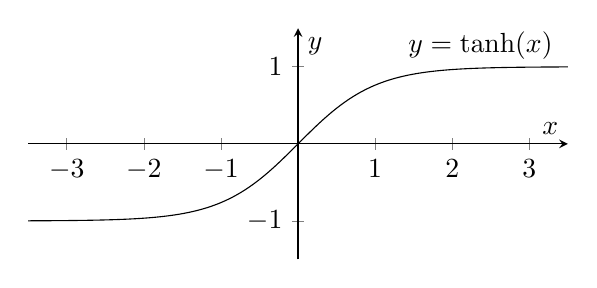
\begin{tikzpicture}[>=stealth]
            \begin{axis}[
                axis equal image,
                xmin=-3.5,xmax=3.5,
                ymin=-1.5,ymax=1.5,
                axis x line=middle,
                axis y line=middle,
                axis line style=->,
                xlabel={$x$},
                ylabel={$y$},
                ]
                \addplot[no marks,black,-] expression[domain=-5:5,samples=1000]{tanh(x)} 
                            node[pos=0.65,anchor=south west, yshift=0.1cm]{$y=\tanh(x)$}; 
            \end{axis}
        \end{tikzpicture}
        \caption{Plot of the function $y=\tanh(x)$.}
    \end{figure}

    As it turns out, the analysis of such MLPs with non-linear activations is much harder.

    \begin{example}
        MLPs with non-linear activations like $\tanh(x)$ can represent non-injective functions (other than $f(x) \equiv \bm{0}$) even when only using one input node.
        
        For instance, the MLP depicted in figure~\ref{fig:non_injective_mlp_single_input} implements the non-injective mapping depicted in figure~\ref{fig:non_injective_function}.

        \begin{figure}[h]
            \centering
            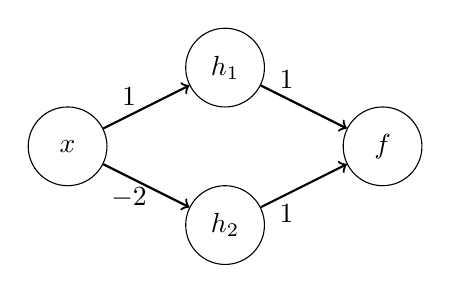
\begin{tikzpicture}[
                    neuron/.style={circle, draw=black, minimum size=1cm},
                    layer/.style={node distance=1.5cm and 2cm},
                    every edge/.style={draw,->,thick}
                ]

                % Input Layer
                \node[neuron] (I1) at (0,0) {$x$};

                \node[neuron] (H1) at (2, 1) {$h_1$};
                \node[neuron] (H2) at (2, -1) {$h_2$};

                % Output Layer
                \node[neuron] (O1) at (4, 0) {$f$};

                % Connections with weights
                \draw (I1) edge node[pos=0.3, above] {$1$} (H1);
                \draw (I1) edge node[pos=0.3, below] {$-2$} (H2);
                \draw (H1) edge node[pos=0.3, above] {$1$} (O1);
                \draw (H2) edge node[pos=0.3, below] {$1$} (O1);
            \end{tikzpicture}
            \caption{Simple MLP using $\tanh(x)$ activation implementing a non-injective mapping.}
            \label{fig:non_injective_mlp_single_input}
        \end{figure}

        \begin{figure}[h]
        \centering
            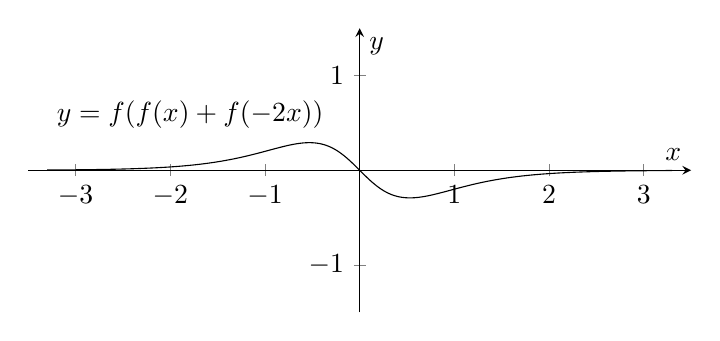
\begin{tikzpicture}[>=stealth]
                \begin{axis}[
                    axis equal image,
                    width=10cm,
                    xmin=-3.5,xmax=3.5,
                    ymin=-1.5,ymax=1.5,
                    axis x line=middle,
                    axis y line=middle,
                    axis line style=->,
                    xlabel={$x$},
                    ylabel={$y$},
                    ]
                    \addplot[no marks,black,-] expression[domain=-3.3:3.3,samples=1000]{tanh(tanh(x) + tanh(-2 * x))} 
                                node[pos=0,anchor=south west, yshift=0.4cm]{$y=f(f(x) + f(-2x))$}; 
                \end{axis}
            \end{tikzpicture}
            \caption{Plot of the function $y=f(f(x) + f(-2x))$ with $f(x) \coloneqq \tanh(x)$.}
            \label{fig:non_injective_function}
        \end{figure}
    \end{example}

    \subsubsection{Multiple Input Nodes}
    As one might expect, the situation gets even more complicated when considering multiple input nodes. Still, we can observe interesting learning behavior of MLPs and examine how their tendency to abstract functions match to those of humans.

    One illustrative example given in the book is to train a MLP with four binary input and output neurons to learn the identity mapping. For example, 1010 is mapped to 1010, 0001 to 0001, and so on. As we can see, this mapping has a finite domain of 16 possible inputs. It would be interesting to analyze how the MLP generalizes when trained on a real subset of the \emph{input space}.

    Let's analyze the case of only training the MLP with inputs where the last bit is 0. Formally, our training data set $\mathcal{D}$ reads as:
    \[
        \mathcal{D} = \{ (\bm{x}, \bm{x}): \bm{x} \in \{0, 1\}^4, \ \bm{x}_4 = 0 \} \quad .
    \]

    \begin{example}
        When you are presented the pattern

        \begin{table}[h]
            \centering
            \begin{tabular}{c|c}
                Input & Output \\
                \hline
                1010 & 1010 \\
                0100 & 0100 \\
                1110 & 1110 \\
                0000 & 0000 \\
            \end{tabular}
        \end{table}
        and asked to predict the output of 1111, many would predict 1111. Note that there is no right or wrong, as potentially any of the 16 possible bit strings are valid. However, we can infer some information about the human bias, which we can use to examine our models.
    \end{example}

    Similarly, after training is completed, we can test what the networks prediction would be for inputs like 1111, which it has never seen before. Interestingly, it predicts 1110. I mean, can we blame it, as it never learned how to handle the last bit. But that is exactly the point: The network could alternatively generalize the behavior it learned for the other three nodes to the last one, but instead it treats them independently. This, essentially, represents a bias of the architecture, which for some tasks (like this one) might be unwanted.

    % \subsection{Conclusion}
    % We suspect brains to work fundamentally different than MLPs: they work recurrently, and learn dynamically without needing to construct entire neural networks for every task. However, the expressive power of MLPs and similar feedforward networks allows them to emulate specific tasks we humans are naturally good at (language, image recognition, etc.). When we train them on a subset of the input domain, these models seem to be chronically bad at generalizing.
    
    % The argument is that this bias misalignment between us humans and these models lies in the architectural design of these models: They are a bare framework described by and processing numbers without any a priori information about the world or the task at hand encoded into them. Of course, engineers try to integrate domain specific knowledge into the architectural design of neural networks, like convolutional layers which aim to recognize shift-invariant features in a 2D image.

    % Personally, I don't think we should try to model the brain by individual neural networks for specific tasks, because for every such task, we would have to construct an architecture that aligns well with the human bias. Instead, we should focus on building one universal model, maybe consisting of different submodels, just like a computer consists of a cpu, gpu, ram etc. This model should have basic computational abilities, and should be able to coordinate and use its different parts in order to effectively handle a variety of tasks. I believe that this diversity of tasks this model can perform reinforces its precision, as it might combine knowledge from different areas.
    
    % Of course, this task is monumentally difficult, but the possibilities of this \emph{artificial general intelligence} are endless, as we can scale those systems and deploy them constantly, hence might be able to operate much more efficiently than humans. The challenge is to find a suitable architecture. However, we have to keep in mind the fundamental differences of the human brain and a digital computer, like the fact that the brain consists of countless individual parallel processing units.

    \subsection{Conclusion}
    We suspect that brains operate fundamentally differently from MLPs. Unlike feedforward networks, brains function recurrently and learn dynamically, without needing to construct distinct neural architectures for every task. However, the expressive power of MLPs and similar feedforward models allows them to emulate specific tasks at which humans excel—such as language processing and image recognition. When trained on a subset of the input domain, these models often perform poorly at generalization.

    The argument is that this misalignment in inductive bias between humans and such models stems from their architectural design. Neural networks are abstract mathematical frameworks that process numbers, with no built-in prior knowledge of the world or the task. While engineers do attempt to incorporate domain-specific knowledge—such as using convolutional layers to recognize shift-invariant features in 2D images—these additions remain narrow in scope.

    Personally, I don't believe we should model the brain by designing individual neural networks for specific tasks, as this would require tailoring an architecture for each task that aligns well with human biases. Instead, we should aim to build a single universal model—possibly composed of modular subcomponents—analogous to how a computer includes a CPU, GPU, RAM, and other parts. Such a model should possess basic computational abilities and be capable of coordinating and utilizing its different components to handle a wide range of tasks. In fact, the diversity of tasks this model can perform may enhance its precision, as it could integrate knowledge across domains.

    Of course, developing such a system is monumentally difficult. But the potential of this form of \emph{artificial general intelligence} is vast: we can scale and deploy these systems continuously, potentially allowing them to operate more efficiently than humans. The central challenge lies in discovering an appropriate architecture—while always keeping in mind the fundamental differences between the human brain and digital computers, such as the massively parallel nature of biological neural processing.
\end{document}
